\documentclass{beamer}

\mode<presentation> 
{
    \usetheme{Madrid}
}

\usepackage[utf8x]{inputenc}
\usepackage[english,russian]{babel}
\usepackage[T2A]{fontenc}
\usepackage{graphicx}
\usepackage{booktabs} 
\usepackage{mathtools}
\usepackage{amsmath}
\usepackage{wasysym}
\usepackage{subfig}
\usepackage{hyperref}
\usepackage{ulem}
\usepackage{ragged2e}
\usepackage{algorithm2e}
\usepackage{minted}


\DeclarePairedDelimiter\ceil{\lceil}{\rceil}
\DeclarePairedDelimiter\floor{\lfloor}{\rfloor}


\usemintedstyle{borland}

\usefonttheme[onlymath]{serif}

\hypersetup
{
    colorlinks=true,
    linkcolor=white, 
    urlcolor=cyan
}

\title[Лекция 5]
{
    Лекция 5: Структуры в языке Си и простейшие структуры данных (стек и очередь)
} 


\author[Д. А. Караваев]{Д. А. Караваев}

\institute[СПбГУТ] 
{
    Санкт-Петербургский государственный университет телекоммуникаций \\ им. проф. М. А. Бонч-Бруевича \\ 
    \vspace{0.2cm}
    Факультет РТС, Кафедра РОС \\
    \vspace{0.2cm}
    Факультатив <<Программирование в ЦОС>> \\
    \vspace{0.2cm}
    Осень 2019
}

\date[18.11.2019]{18.11.2019 Санкт-Петербург} 

\begin{document}
    \begin{frame}
        \titlepage 
    \end{frame}
    \begin{frame}[fragile]
        \frametitle{Структуры в языке Си}
        \justifying
        В языке Си существует возможность создать свой собственный {\it тип} (пользовательский) данных на основе композиции из уже существующих типов. Такая композиция называется {\bf структурой}. Части структуры называются {\bf полями}.
        \begin{minted}[frame=lines,         framesep=2mm,
                       baselinestretch=1.2, fontsize=\footnotesize,
                       linenos]{c}
/* Объявление структуры, задающей комплексное число: */
struct complex_t
{
    double re; /* Поле: вещественная часть. */
    double im; /* Поле: мнимая часть. */
};
/* Создание переменной типа complex_t */
struct complex_t x;
/* Обращение к полям структуры: */
x.re = 1.4; 
x.im = 2.1245;
        \end{minted}
    \end{frame}
    \begin{frame}[fragile]
        \frametitle{Функции от структур}
        \justifying
        Для типа {\tt struct complex\_t} не определена ни одна операция. Все операции над данным типом необходимо реализовывать через {\it функции}.
        \begin{minted}[frame=lines,         framesep=2mm,
                       baselinestretch=1.2, fontsize=\footnotesize,
                       linenos]{c}
/* Вычисление модуля в квадрате: */
double complex_abs2(struct complex_t x)
{
    return x.re * x.re + x.im * x.im;
}
/* Вычисление суммы двух комплексных чисел: */
struct complex complex_sum(struct complex_t lhs, struct complex_t rhs)
{
    /* Создание и инициализация: */
    struct complex result = {.re = lhs.re + rhs.re, 
                             .im = lhs.im + rhs.im}; 
    return result;
}
        \end{minted}
    \end{frame}
    \begin{frame}[fragile]
        \frametitle{Функции от структур}
        \justifying
        Для типа {\tt struct complex\_t} неопределена ниодна операция. Все операции над данным типом необходимо реализовывать через {\it функции}.
        \begin{minted}[frame=lines,         framesep=2mm,
                       baselinestretch=1.2, fontsize=\footnotesize,
                       linenos]{c}
/* Вычисление модуля в квадрате: */
double complex_abs2(struct complex_t x)
{
    return x.re * x.re + x.im * x.im;
}
/* Вычисление суммы двух комлексных чисел: */
struct complex complex_sum(struct complex_t lhs, struct complex_t rhs)
{
    /* Создание и инициализация: */
    struct complex result = {.re = lhs.re + rhs.re, 
                             .im = lhs.im + rhs.im}; 
    return result;
}
        \end{minted}
    \end{frame}
    \begin{frame}[fragile]
        \frametitle{Указатели на структуру}
        \justifying
        \begin{minted}[frame=lines,         framesep=2mm,
                       baselinestretch=1.2, fontsize=\footnotesize,
                       linenos]{c}
/* Объявление с typedef чтобы избежать использование struct: */
typedef struct 
{
    complex_ t samples[1000]; /* Поле: массив с отсчётами. */
    size_t     N; /* Поле: реальная длина сигнала. */
    /* Различные метаданные ... */
} signal_t; /* Имя типа. */
/* Передача в функцию через указатель (во избежание копирования): */
double signal_mlp_const(double value, signal_t* signal)
{
    for (size_t n = 0; n < signal->N; ++n)
    {
        signal->samples[n] *= value; /* Обращение через ->. */
    }
}
        \end{minted}
    \end{frame}
    \begin{frame}[fragile]
        \frametitle{Указатели на структуру}
        \justifying
        \begin{minted}[frame=lines,         framesep=2mm,
                       baselinestretch=1.2, fontsize=\footnotesize,
                       linenos]{c}
/* const указатель для выделения входного параметра: */
double signal_energy(const signal_t* signal)
{
    double sum = 0.0;
    for (size_t n = 0; n < signal->N; ++n)
    {
        sum += complex_abs2(signal->values[n]);
    }
    return sum / signal->N;
}
/* Создание: */
signal_t signal;
/* Инициализация ... */
signal_energy(&signal); /* Вызов. */
        \end{minted}
    \end{frame}
    \begin{frame}[fragile]
        \frametitle{Структуры в Си}
        \justifying
        {\bf Вывод}: структура ({\it данные}) и функции направленные на работу с ней ({\it методы}) формируют пользовательский тип ({\bf класс}), оперирование с которыми лежит в основе парадигмы {\it объектно-ориентированного программирования} (ООП).
        \begin{minted}[frame=lines,         framesep=2mm,
                       baselinestretch=1.2, fontsize=\footnotesize,
                       linenos]{c}
/* Данные: */
typedef struct 
{
    /* ... */
} signal_t;
/* Методы: */
double signal_energy(const signal_t* signal);
uint64_t signal_duration_nanos(const signal_t* signal);
void signal_correlate(const signal_t* lhs, const signal_t* rhs, 
                            signal_t* result);
/* ... */
        \end{minted}
    \end{frame}
    \begin{frame}
        \frametitle{Стек и очередь}
        \begin{block}{Структуры данных}
            \justifying
            Способ организации однотипных данных в памяти, удовлетворяющий некоторому интерфейсу a.k.a {\it Application Programming Interface} ({\bf API}).
        \end{block}
        \begin{block}{Очередь}
            \justifying
            Набор элементов одного типа, в который можно поместить элемент и взять {\it первый} помещенный. "Честная"\ очередь. Принцип First-In-First-Out ({\bf FIFO}).
        \end{block}
        \begin{block}{Стек (стопка)}
            \justifying
            Набор элементов одного типа, в который можно поместить элемент и взять {\it последний} помещенный. "Нечестная"\ очередь. Принцип Last-In-First-Out ({\bf LIFO}).
        \end{block}
    \end{frame}
    \begin{frame}
        \frametitle{Иллюстрация очереди и стека}
        \begin{figure}[!tbp]
           \centering
           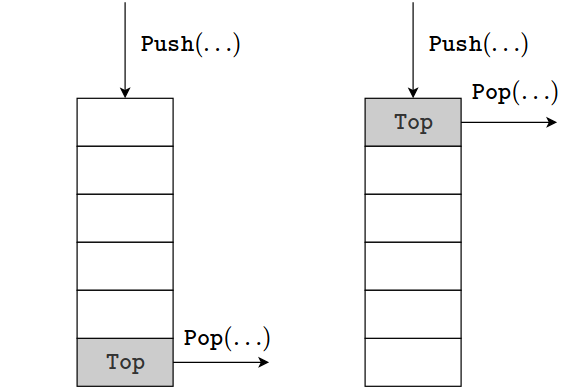
\includegraphics[width=0.8\textwidth]{pics/sq.png}
       \end{figure}
    \end{frame}
    \begin{frame}[fragile]
        \frametitle{Задание}
        Реализовать:
        \begin{enumerate}
            \item {\tt Push}$(\dotsc)$ - поместить элемент (целое число) в очередь (стек);
            \item {\tt Pop}$(\dotsc)$ - удалить элемент из очереди (стека);
            \item {\tt Top}$(\dotsc)$ - вернуть "первый"\ элемент очереди (стека);
            \item {\tt Full}$(\dotsc)$ - проверка на полноту очереди (стека);
            \item {\tt Size}$(\dotsc)$ - вернуть число элементов очереди (стека).
        \end{enumerate}
        \vspace{0.5cm}
        \par
        \justifying
        {\bf Замечание}: На самом деле поведение стека и очереди совпадают с точностью до реализации методов  {\tt Push}$(\dotsc)$ и  {\tt Pop}$(\dotsc)$.
    \end{frame}
    \begin{frame}[fragile]
        \frametitle{Структуры для стека и очереди}
        \begin{minted}[frame=lines,         framesep=2mm,
                       baselinestretch=1.2, fontsize=\footnotesize,
                       linenos]{c}
/* Структура для стека: */
typedef struct
{
    int    values[100]; /* Элементы. */
    size_t size; /* Число элементов. */
    int    top; /* Индекс первого элемента. */ 
} stack;
/* Структура для очереди: */
typedef struct
{
    int    values[100]; /* Элементы. */
    size_t size; /* Число элементов. */
    int    top; /* Индекс первого элемента. */ 
} queue;
        \end{minted}
    \end{frame}
    \begin{frame}
        \begin{center}
        \baselineskip 20.0mm
        \Huge Спасибо за внимание!
        \end{center}
    \end{frame}
\end{document}
